\chapter{Overview of the tool Storm}
\textit{This chapter is essentially based on the article named ``A Storm is coming: a modern probabilistic model checker'' \cite{storm1} and on the documentation of the tool.} \\

Storm is a probabilistic model checker recently released. It is able to analyse
four Markov models, featuring discrete-time Markov chains and Markov decision processes. The main aim of this tool is to be competitive in terms of performances, to be updated with new verification algorithms, to be able to
deal with a large panel of modeling languages,... This tool provides %many other
a lot of model checking features, including solvers for problems presented in the previous chapter and
for multi-objective problems. In this chapter, we will briefly present how our MDPs can be defined in this powerful tool, how they are represented and with which different approaches problems are solved.
Whit this background, we will enrich next chapters with practical Storm examples.

\section{Models}
As mentioned above, Storm allows to model-check four types of Markov models.
The first family of models is discrete-time Markov models, that are covered in the first chapter, composed by
discrete-time Markov chains and Markov decision processes.
The second family of models is continuous-time Markov models, composed by continuous-time Markov chains and Markov automata. \\

Continuous-time Markov chains models (CTMC) \cite{maro} are similar to discrete-time Markov chains, but each state $s$ is
characterised by an exit rate $\lambda_s$.
The time $t$ spent in each state $s$ of the system is negatively exponentially distributed with this rate, i.e., the probability to stay in $s$ after $t$ time units passed in $s$ is $e^{- \lambda_s t}$.
This exit rate and a probability transition function allow to induce a generator
function with which it is possible to compute the probability
%to go from one state to another after a certain time.
that the system is currently in a state $s'$ while the system was in the state $s$, $t$ time units ago.
Note that the ``step'' notion is replaced by the ``time'' notion in comparison with discrete-time models. Furthermore, a Markov automata (MA) is a continuous-time nondeterministic Markov model where the key idea is the same as between MCs and MDPs in discrete-time. \\

We will not dwell on continuous-time models anymore and focus primarily on discrete-time models.

\section{Input formats}
Storm supports various native input formats, including Prism, Jani, generalised stochastic Petri nets, dynamic fault trees, cpGCL and explicit format.
We will introduce the three input languages supported by the main executable of Storm by presenting how to use them to model our
discrete-time systems.
\subsection{Prism} \label{prism-subsec}
The Prism language \cite{prismsynt} allows to deal with MCs, CMCs and MDPs in Storm.
It is a state-based language using reactive \textit{modules}.
We will not define the complete syntax and semantic of the Prism language, but rather provide a way to
define our MDPs.
Let $\mathcal{M} = (S, A, \Delta, w, AP, L)$ be a finite MDP, with $|S| = n$, and $s_i \in S$ be the $i^{\text{th}}$ state of $S$ from which events that we are
interested to measure start, with $i \in \{0, \dots, n-1\}$. \\

In the Prism language, a \textit{module} represents a component of the system.
By definition of our MDPs, we just need a single module to
represent them. A module allows to characterise $S$, $A$ and $\Delta$. We begin by enumerating states of $\mathcal{M}$:
\[
  x: [0\, ..\, n-1] \; \text{init} \; i;
\]
In the Prism language, $x$ is considered as a \textit{variable} of the module, ranging on states of $\mathcal{M}$.
In this manner, we express that for all $j \in \{0, \dots, n-1\}$, $s_j \in S$
is the $j^{\text{th}}$ state of $S$ represented by the index $j$ of the variable $x$ (i.e., $x=j$), and $s_i$ is the initial state from which events start, represented by the index $i$ of the variable $x$ (i.e., $x=i$).
Note that a variable represents a set of states of the MDP. Thus, it is possible that a module has more than one variable if the state space of the MDP is formed by a Cartesian product of set of states.
Thanks to variables of the module, it is possible to form predicates $\Phi$ on the variables of the module with the syntax described with the following grammar:
\begin{align*}
  \Phi &::= true \; | \; x \varphi p \; | \; (X) \; | \; (\Psi) \\
  X &::= \Phi \; | \; \Phi \& X \\
  \Psi &::= \Phi \; | \; \Phi || \Psi
\end{align*}
where $x$ is a variable of the module, $\varphi \in \{<, \leq, >, \geq, =, \neq\}$
and $p \in \mathbb{N}$. Let $s \in S$ be a state of $\mathcal{M}$. We have that $s \models \Phi$ iff $\Phi$ is true for the state $s$, i.e.,
\begin{itemize}
  \item $s \models true$,
  \item $s \models x \varphi p$ iff there exists an index $j \in \mathbb{N}$ in the range of indices of the module variable $x$ by which the state $s$ is represented (i.e., $s$ is represented by $x=j$) and such that $j \varphi p$.
  \item $s \models (\Phi_1 \& \dots \& \Phi_m)$ iff
    for all $k \in \{1, \dots, m\}$, $s \models \Phi_k$, and
  \item $s \models (\Phi_1 || \dots || \Phi_m)$ iff
    there exists $k \in \{1, \dots, m\}$ such that $s \models \Phi_k$.
\end{itemize}
We denote by $Sat(\Phi)$ the set of states satisfying the predicate $\Phi$, i.e., $Sat(\Phi) = \{s \in S \; | \; s \models \Phi\}$.

\begin{example}[\textit{Satisfaction of a predicate on variables of an MDP module}] Consider an MDP $\mathcal{M}$ with state space $S$ and a Prism program containing a module $M$ defining this MDP.
Assume that the size of the state space $S$ is $|S| = 5$ and that the module $M$ contains an unique variable $x$, ranging on all states of $S$. Let
$\Phi = (x \leq 1 \,||\, x >3)$ be a predicare on the variables of the module $M$, then $Sat(\Phi) = \{s_0, s_1, s_4\}$.
\end{example}

The behaviours of the module, i.e., transitions of the set $\rightarrow$\footnote{remind that the transition relation $\rightarrow$ is the set $\{ (s, \alpha, s') \in S \times A \times S \; | \; \Delta(s, \alpha, s') > 0 \}$} are then described
inside the module by a set of \textit{guarded commands}, taken the following form:
\[
  [\alpha] \; \Phi \rightarrow \delta_1: \phi_1 + \dots + \delta_m: \phi_m;
\]
where $\Phi$ is a predicate over the variables of the module such that, for all $s \in Sat(\Phi)$, $\alpha \in A(s)$, $i \in \{1, \dots, m\}$, $\delta_i \in [0, 1]$ with $\sum_{i=1}^m \delta_i = 1$ and where $\phi_i$ is an \textit{update formula} describing a state represented by a variable of the module. This guarded command basically means that all states that satisfy the predicate $\Phi$ go to the state  described by $\phi_i$ with a probability $\delta_i$, when the action $\alpha$ is chosen.
An update formula $\phi$ is of the form
\[\phi::=(x'_1=u_1) \& (x'_2=u_2) \& \dots \& (x'_k=u_k)\]
where $x_1, x_2, \dots, x_k$ are variables of the module and $u_1, u_2, \dots, u_k$ are \textit{expressions} (i.e., literal values, variables, constants and operators) over all variables.
% \begin{align*}
%   \phi &::= (s'=\chi) \; | \; (s'= \mu(\chi, \chi)) \; | \; \psi \\
%   \chi &::= s \varphi x \; | \; x \\
%   \psi &::= \phi \; | \; \phi \& \psi
% \end{align*}
% where $s$ is a variable of the module,
% $\varphi \in \{+, -\}$, $\mu \in \{\min, \max \}$ and $x \in \mathbb{N}$.
% Let assume that the system is currently in the $j^\text{th}$ state of $S$, i.e.,
% in the state $s_j$
% %The expression $\chi$ actually represents the core of a variable update ; it represents the index of the state to which the system evolves.
% %\begin{itemize}
% %  \item $\chi = x$ directly refers to the index $x$ of the variable to update and
% %  \item $\chi = s \varphi x$ refers to the current index of the variable $s$ on which the operation $\varphi x$ is applied (here, $j \varphi x$).
% %\end{itemize}
% and let $k \in \{0, \dots, n-1\}$. We have that $s_k \models \phi$ iff $\phi$ refers to the state $s_k$, i.e.,
% \begin{itemize}
%   \item $s_k \models s' = x$ iff $k = x$. Then the system go from $s_j$ to $s_x$.
%   \item $s_k \models s' = s \varphi x$ iff $k$ is the current index of the variable $s$ on which the operation $\varphi$ has been applied. Here, we have $k = j \varphi x$. Thus the system go from $s_j$ to $s_{j+\varphi}$.
% \end{itemize}
\begin{example}[\textit{Guarded command for a simple module}]
Let $\mathcal{M}$ be an MDP with state space $S$. Consider that all states of $\mathcal{M}$ are represented by the values of the single variable $x$, ranging on all states of the set $S$, with $|S|=n$, the transitions of $\mathcal{M}$ can be described with the following guarded command:
let $s_j$ be the $j^{\text{th}}$ state of $S$, for all enabled actions $\alpha \in A(s_j)$ of $s_j$,
\[
  [\alpha] \; x=j \rightarrow \delta_0: x'=j_0 + \dots + \delta_{m-1}:  x'=j_{m-1};
\]
where $s_{j_0}, \dots, s_{j_{m-1}}$ are $\alpha$-successors of $s_j$ and $\delta_k = \Delta(s_j, \alpha, s_{j_k})$,
with  $m=|Succ(s_j,\alpha)|$, $k \in \{0, \dots, m-1\}$, $j_k \in \{0, \dots, n-1\}$ and where $s_{j_k}$ is the $k^\text{th}$ $\alpha$-successor of $s_j$ and the $j_k^\text{th}$ state of $S$.
\end{example}

The set of atomic propositions $AP$ and the labelling function $L$ of $\mathcal{M}$ are characterised in the Prism language as follows: for all $a \in AP$,
\[
  \text{label} \; ``a" = \Phi;
\]
where the set of states satisfying the predicate $\Phi$ is actually the set of states labelled with $a$, i.e., $Sat(\Phi) = \{ s \in S \; | \; a \in L(s) \}$. \\

% \[
%   \text{label} \; ``a" = (s=j_0\, \& \, \dots \, \& \, s=j_{m-1});
% \]
% where $S_a= \{s \in S \; | \; a \in L(s) \}$ and $s_{j_k} \in S_a$,
% with $m = |S_a|$, $k \in \{0, \dots, m-1\}$,
% $j_k \in \{ 0, \dots, n-1 \}$ and $s_{j_k}$, the $k^\text{th}$ state of $S_a$ and the $j_k^\text{th}$ state of $S$.
%

Finally, the weight function $w$ can be characterised with the notion of \textit{rewards}. In the Prism language, it is possible to associate to each transition
of the set %$\{ (s, \alpha, s') \in S \times A \times S \; | \; \Delta(s, \alpha, s') > 0 \}$
$\rightarrow$
a real value. A \textit{dimension rewards} is a set of rewards that take the following form:
\[
  [\alpha] \; \Phi: x;
\]
where $\alpha \in A$ is an action, $\Phi$ is a predicate and $x \in \mathbb{R}$
is the value of the reward of going from a state $s \in S$, such that $\alpha \in A(s)$, to states of $Sat(\Phi)$. Note that if the action $\alpha$ is omitted (giving a reward of the form $[]\; \Phi: x^*;$), each transition $s \xrightarrow{\,\alpha\,} s'$ such that $s' \in Sat(\Phi)$ and $\alpha \in A(s)$
has a reward of $x^*$. Note also that it is possible to specify multiple dimensions rewards for an MDP. We will detail this notion later.
We can adapt the reward notion to describe the weight function of our MDPs with a set of rewards formed as follows:
let $\alpha \in A$ be an action of $\mathcal{M}$ and $x = w(\alpha)$, the reward formed by
\[
  [\alpha] \; true: x;
\]
is actually the weight of the action $\alpha$.

\begin{example}[\textit{Define an MDP in the Prism language}]
Let $\mathcal{M}=(S, A, \Delta, w, AP, L)$ be the MDP of Figure \ref{prism-simple}. This MDP can be defined in the Prism language as follows:\\
\begin{minipage}{0.4\linewidth}
  \lstinputlisting[language={Prism},
      rulesepcolor=\color{black}, rulecolor=\color{black},
      breaklines=true,
      breakatwhitespace=true, firstnumber=1, firstline=1, lastline=25]{resources/simple_mdp.prism}
\end{minipage}
\begin{minipage}{0.6\linewidth}
    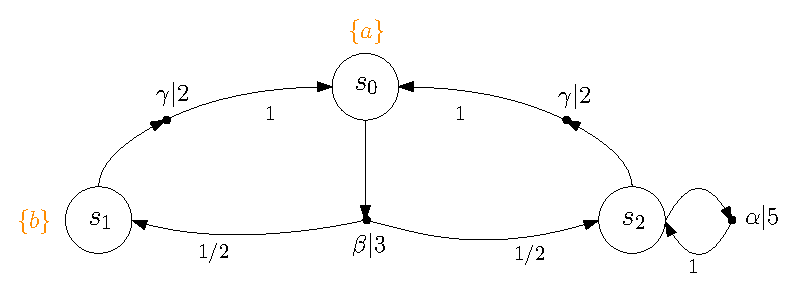
\includegraphics[width=\linewidth]{resources/simple-mdp}
    \captionsetup{justification=centering}
    \captionof{figure}{MDP $\mathcal{M}$, with $S = \{s_0, s_1, s_2\}$, $A = \{\alpha, \beta, \gamma\}$ and $AP = \{a, b\}$}\label{prism-simple}
\end{minipage}
\end{example}

\begin{example}[\textit{Unfold an MDP in the Prism language}]
Let $\mathcal{M}=(S, A, \Delta, w, AP, L)$ be the MDP of Figure \ref{prism-simple} and $l \in \mathbb{N}$
be a length threshold such that $l=8$. We can define the unfolding of $\mathcal{M}$ from the state $s_0$ until the length threshold $l$ for the set of target states $T = \{s_1\}$ (cf. figure \ref{unfolding}) in the Prism language as follows:
\lstinputlisting[language={Prism},
    rulesepcolor=\color{black}, rulecolor=\color{black}, breaklines=true,
    breakatwhitespace=true, firstnumber=1, firstline=1, lastline=25]{resources/unfolded_simple_mdp.prism}
\end{example}
Since the state space of the unfolded MDP $\mathcal{M}_l$ is a Cartesian product between the state space $S$ of $\mathcal{M}$ and the set $V = \{0, \dots, l, \bot\} \subseteq \mathbb{N} \cup \{\bot\}$, we can define the variables of the unfolded MDP $\mathcal{M}_l$ with the variables of $\mathcal{M}$ and a new variable $v$, ranging from $0$ to $l+1$ (where the $(l+1)^\text{th}$ state actually represents the $\bot$ value). The guarded
commands of the module are obviously defined, following the definition of the
probability transition function $\Delta_l$ of any unfolded MDP. Finally, a label $target$ is added,
labelling each state of the set $T_l = \{ (t, v) \in S \times V \; | \; t \in T \; \wedge \; v \leq l \}$.

\subsection{Explicit format}
Storm also supports input models specified in explicit format. The syntactic power of such a format is lower compared to the Prism language, but is
very simple and intuitive. Thereby, this format can thus be interesting in case of
we want to verify a model generated from another tool (e.g., MRMC or Prism).
In general, a same model generated in explicit format from different tool does not match exactly. However, it can be easily modified by hand to be handled by Storm due to
the simplicity of the format. \\

An MDP specified in explicit format
consists of a transitions matrix file, describing explicitly transitions of the system, a reward matrix file, describing explicitly
rewards of these transitions, and a labelling set file. More formally, let $\mathcal{M} = (S, A, \Delta, w, AP, L)$ be a finite MDP, where $|S| = n$ and where $A(s)$ is countable for all $s \in S$. The transition matrix $P$ and the rewards matrix $R$ of sizes $(|\rightarrow|, 4)$ are defined as follows:
let $l \in \{1, \dots, |\rightarrow|\}$ be the $l^\text{th}$ line of $P$ and $R$,
\begin{itemize}
  \item $P_{l, 1} = R_{l, 1}$ is the index $i$ of the source state $s_i \in S$ of the $l^\text{th}$ transition of $\rightarrow$,
  \item $P_{l, 2} = R_{l, 2}$ is the index $k$ of an enabled action of $s_i$ in $A(s_i)$,
  \item $P_{l, 3} = R_{l, 3}$ is the index $j$ of the target state $s_j \in S$ of this transition and
  \item $P_{l, 4}$ is the nonzero transition probability $p$ given by $\Delta(s_i, \alpha_{s_i, k}, s_j)$, where $\alpha_{s_i, k}$ denotes the $k^\text{th}$ enabled action of $A(s_i)$.
  \item $R_{l, 4}$ is the reward of the transition $(s_i, \alpha_{s_i, k}, s_j)$.
\end{itemize}
Thus, the line $l \in \{1, \dots, |\rightarrow|\}$ of $P$ defined by the vector $(i, k, j, p) \in \mathbb{N}^3
\times [0, 1]$ describes that the state $s_i$ goes to the state $s_j$ by choosing
the $k^\text{th}$ enabled action $\alpha_{s_i, k}$ of $A(s_i)$ with a probability $p = \Delta(s_i, \alpha_{s_i, k}, s_j)$. In a similar way,
the line $l' \in \{1, \dots, |\rightarrow|\}$ of $R$ defined by the vector
$(i, k, j, r) \in \mathbb{N}^3 \times \mathbb{R}$ describes that the state $s_i$ goes to the state $s_j$ by choosing the $k^\text{th}$ enabled action $\alpha_{s_i, k}$ of $A(s_i)$ with a reward $r$.
Since rewards of our MDPs are actually costs of actions, this reward $r$ equals $w(\alpha_{s_i, k})$. \\

Finally, labels of this MDP are defined with a set of vectors $L_\text{explicit}$ defined as follows : \[L_\text{explicit} = \{(i, a_1, \dots, a_k) \in \mathbb{N} \times AP^k \; | \; k = |L(s_i)| \wedge \{a_1, \dots, a_k\} = L(s_i)\}\]

\begin{example}[\textit{Define an MDP in explicit format}]
Let $\mathcal{M}=(S, A, \Delta, w, AP, L)$ be the MDP of the figure \ref{prism-simple}. The explicit transition matrix $P$, the explicit reward matrix $R$ and the explicit set of labels $L_\text{explicit}$ of $\mathcal{M}$ are defined as follows :
  \begin{equation*}
  P =
  	\begin{pmatrix}
  	0 & 0 & 1 & \frac{1}{2} \\[0.3em]
  	0 & 0 & 2 & \frac{1}{2} \\[0.3em]
  	1 & 0 & 0 & 1 \\[0.3em]
    2 & 0 & 2 & 1 \\[0.3em]
    2 & 1 & 0 & 1
  	\end{pmatrix}, \quad \quad
  R =
    \begin{pmatrix}
  	0 & 0 & 1 & 3 \\[0.3em]
  	0 & 0 & 2 & 3 \\[0.3em]
  	1 & 0 & 0 & 2 \\[0.3em]
    2 & 0 & 2 & 5 \\[0.3em]
    2 & 1 & 0 & 2
    \end{pmatrix}, \quad \quad
  L_\text{explicit} = \{ (0, a), (1, b) \}
  \end{equation*}
\end{example}

\subsection{Jani}
Jani \cite{JQM} is a recent modeling language whose syntax is based on Json and whose design is based on networks of communicating automata.
The purpose of this language is to provide a stable and uniform interface
between tools and, more particularly, model checkers.
This format supports MCs, CTMCs, MDPs and MAs. \\

Actually, the semantic model of the Prism language forms the conceptual basis of
Jani and is extended to also support MAs.
Furthermore, Jani is designed to be more trivial than the Prism language and, thus,
to be easy to generate and parse programmatically without library dependencies.
However, Jani has not been designed to be created manually by users, but rather
to be automatically generated from higher-level and domain-specific languages, while remaining human-readable, in contrast to binary encodings. Storm actually allows to
convert multiple input types to Jani. An example of conversion in available in appendix (cf. appendix \ref{prism2jani}).

\section{Properties}
Storm uses \textit{probabilistic branching time logic}, i.e., PRCTL and CSL,
to verify respectively properties of discrete-time and continuous-time models.
We will focus on PRCTL in the next chapter (cf. sections \ref{PRCTL-MC} and \ref{PRCTL-MDP}).
We will see that the language of such a logic additionally allows to formulate requests to solve problems encountered in the first chapter and for problems we will encounter later.

%\section{Implementation}
\section{Engines}
Storm is decomposed in five engines that pursue different approaches to solve a problem.
\begin{itemize}
  \item \textit{Sparse}: this engine is the default one. It uses sparse matrices as in-memory representation of models. Numerical analysis methods allow efficient memory allocation and fast operations for this data structure on small and moderately sized models.
  Actually, this data structure is very powerful in the case of most states of the model have transitions to a small subset of the set of states of the model. This case represents actually most of the cases: in general, underlying graphs of Markov models are rarely complete and the transitions matrix representing the probability transition function of
  most of the models is thus sparse.
  \item \textit{DD}: this engine uses multi-terminal binary decision diagrams (MTBDDs) as their primal representation. This data structure allows
  to handle gigantic models. Intuitively, each state of the system are encoded on $n$ bits and the probability transition function is a boolean function
  over the bits representation of two states. Binary decision diagrams (BDDs) are
  used to represent boolean functions and are actually compressed binary decision trees through directed acyclic graphs (DAGs), with two terminal states ($1$ and $0$). MTBDDs are BDDs allowing numerical values for terminal states.
  \item \textit{Hybrid}: this engine uses MTBDDs as representation of models, but sometimes uses sparse matrices if operations are judged more appropriate with this format.
  \item \textit{Abstraction refinement}: this engine \textit{abstracts} (non-necessary finite) discrete-time Markov models to finite \textit{stochastic games} and automatically \textit{refines} the \textit{abstraction} as necessary. This engine is suited for models with an infinite state space (other engines cannot handle this type of models).
  \par Intuitively, the abstraction consists of constructing a smaller model by removing details from the concrete system.
  The motivation is that when a property hold in the abstract model, then it also holds in the concrete system.
  If the property does not hold in the abstraction, then either information from the model checking process allow to exhibit a counter-example to show that the property is false in the concrete system, or the abstraction is refined.
  \par Constructing an abstraction of an MDP implies a greater degree of nondeterminism.
  The process of abstraction must maintain a distinction between the nondeterminism from the original MDP and from the nondeterminism induced during the abstraction process, and it is why stochastic games are used \cite{DBLP:journals/fmsd/KattenbeltKNP10}.
  \item \textit{Exploration}: this engine uses sparse representation for models and explores the state space of models with machine learning methods.
\end{itemize}

\section{Solvers}
Several solvers are available in Storm.
Storm uses the suited solver according to the situation (i.e., the input model, its format, the engine used and its in-memory representation).

\begin{itemize}
  \item \textit{Linear equation systems}: Storm provides a
    solver for linear equation systems, allowing to solve reachability and expectation problems in MCs (cf. section \ref{obj-MC} in the first chapter).
  \item \textit{Bellman equations}: these equations form
    systems defined in the next chapter for MDPs (cf. theorem
    \ref{bellman1} and Appendix \ref{bellman2}) whose solutions describe
    reachability and expectation properties.
    The associated solver is based on an approximation technique named \textit{value iteration}, also described in the next chapter.
    Intuitively, this technique approximates values of the solution of the equation by iteratively updating the approximation. This approximation is guaranteed to converge to the solution of the equation system.
    Therefore, the difficulty of this technique is to find a threshold used to stop the iteration process.
    \par Since numerical methods are prone to numerical problems, Storm supports enabling \textit{exact arithmetic} to obtain precise results.
  \item \textit{Linear programming}: a solver for (mixed-integer) linear programs is implemented in Storm, allowing to describe reachability and expectation properties for MDPs, as encountered in the first chapter (cf. subsection \ref{vssp} in the first chapter and the linked LPs in Appendix \ref{LP-app}).\par
  If the size of the considered MDP is sufficiently moderate, Storm uses this solver as the primary.
  \item \textit{SMT}: a SMT problem is a decision problem for first-order logical formulae with equality and without quantifier. SMT solvers are used to minimise the size of models by \textit{bisimulation}.
  A bisimulation is an equivalence relation between two systems having the same behaviour.
  \item \textit{Stochastic games}: although Storm does not support stochastic games as input format,
    solvers for them are available for the abstraction refinement engine
    which uses these as representation.
\end{itemize}
